\section{XQuery}
\label{sect:theory:xquery}

XQuery is a query language developed by the XML Query working group of W3C.
Version 1.0\cite{w3c00} became a W3C Recommendation January 2007. It was designed as a
response to an emerging task: to intelligently express queries in the increasing
amounts of information stored, exchanged and presented using XML. The language
is derived from Quilt\cite{quilt_queryLanguage}.

\begin{itemize}
\item itroduksjon
\item historie
\item bruksomr\aa der
\item ...
\end{itemize}

\subsection{Basics}
\label{sect:theory:basics}
\begin{itemize}
  \item sekvenser og ting atomisk, alt je sekvenser er endimensjonale\ldots
  \item andre ting som er basisk og ikke surt
  \item context item '.'
\end{itemize}

\subsection{Path Expressions}
\label{sect:theory:xqueryPathExpressions}
\begin{itemize}
\item fra XPath / brukt i mange andre ting (XSLT yeye)
\item ...
\item akser -> [Definition: The following axes are designated as optional axes:
ancestor, ancestor-or-self, following, following-sibling, preceding, and
preceding-sibling.] (http://www.w3.org/TR/xquery/\#dt-optional-axis)
\item semantikk 
\item eksikveringsorden etc
\end{itemize}

\subsection{Predicates}
\label{sect:theory:xqueryPredicates}
\begin{itemize}
  \item predikater kan brukes etter b\aa de stepExprz og filterExprz
  \item de gj\o r egentlig ikke noe annet enn \aa~ begrense hva som er i settet
  f\o r (og alt er jo sett)
  \item unntaket er talltingen.. som sikkert er en forkortelse for
  plzReturnTheNumberInTheSequenceIamInRightNow() ellerno.. har ikke lest
  tingen: http://www.w3.org/TR/xquery/\#id-predicates
\end{itemize}

\subsection{FLWOR}
\label{sect:theory:flwor}

\begin{itemize}
\item motiv
\item ...
\item F L W O R semantikk
\item \^{} --- eksikveringsorden etc
\item scoping, hvilke variable er i hvilke scopes (for \$i in \$i..)
\end{itemize}

\subsection{Binary Operators}

\begin{itemize}
\item motiv
\item ...
\item semantikk
\item hva er sant, hva er usant?
\end{itemize}

\subsection{Types}
\begin{itemize}
  \item skrive om dette ogs\aa~selv om vi ikke skal implementere?
  \item har planer om \aa~diskutere det litt i diskusjonskap iallefall..
\end{itemize}

\subsection{Evt andre ting fra XQuery vi kommer til \aa~implementere}

\begin{itemize}
\item if then else

\end{itemize}

\subsection{Full Text Extensions}

\begin{itemize}
\item motiv
\item ...
\item semantikk
\item hva har man? ftcontains er kilden...
\end{itemize}

\subsection{XQuery core}
\label{sect:theory:xqXQcore}
\begin{itemize}
  \item Hva er xquery core?
  \item Hva er poenget med XQuery core?
  \item Normaliseringsprosessen (hva blir til hva)
\end{itemize}

XQuery Core is a less powerful but semantically equivalent form of expressing
XQuery queries. XQuery Core as well as the process of normalizing regular
XQuery to XQuery Core is described in the document ``XQuery 1.0 and XPath 2.0
Formal Semantics''\cite{xquery_semantics}.

The goal of XQuery Core is to simplify queries and remove syntactic sugar,
leaving only the essential semantics without loss of expressiveness.
This is useful for optimization routines and translations into new types of
queries, for example relational algebra or SQL.

The process of normalization is described through a rich set of mapping
rules. These are documented in detail throughout ``XQuery 1.0 and XPath 2.0
Formal Semantics''\cite{xquery_semantics} and will not be reiterated here.
However we will examine some important examples.

First, however, it is important to take note of the syntax of the mapping
rules, as described in \cite{xquery_semantics}, section 3.2.2. 
 
\begin{figure}[!h]
  \centering
$
[Object]_{Subscript}, premises == Mapped Object
$
  \caption{Mapping rules syntax}
  \label{figure:xquery:mapping_rules}
\end{figure}

Consider figure \ref{figure:xquery:mapping_rules}. The left-hand side of the
equality symbol (==) denotes the original object to be rewritten. The
subscript indicates the type or kind of the object to be mapped, and/or
additional information to be passed between mapping rules. The right-hand side
denotes the rewritten object.

\subsubsection{Rewriting FLWOR expressions}

\begin{figure}[!h]
\centering
[for $\$VarName_1$ $OptTypeDeclaration_1$ $OptPositionalVar_1$ in $Expr_1$,
\ldots, $\$VarName_n$ $OptTypeDeclaration_n$ $OptPositionalVar_n$ in $Expr_n$
$FormalReturnClause]_{Expr}$ \newline
$==$ \newline
for $\$VarName_1$ $OptTypeDeclaration_1$
$OptPositionalVar_1$ in $[Expr_1]_{Expr}$ return \ldots for $\$VarName_n$
$OptTypeDeclaration_n$ $OptPositionalVar_n$ in $[Expr_n]_{Expr}$ return
$[FormalReturnClause]_{Expr}$
  \caption{FLWOR expression mapping rule}
  \label{figure:xquery:flwor_mapping_rule}
\end{figure}

The mapping rule for FLWOR forclause-expressions can be seen in figure
\ref{figure:xquery:flwor_mapping_rule}. The mapping rule for LET expressions is
similar and omitted from this document for brevity, however they are also
normalized into several nested bindings.

\begin{figure}[!h]
\centering
$[where Expr_1 FormalReturnClause]_{Expr}$ \newline
$==$ \newline
$if ([Expr_1]_{Expr}) then [FormalReturnClause]_{Expr} else ()$
  \caption{Where-clause mapping rule}
  \label{figure:xquery:where_mapping_rule}
\end{figure}

\begin{figure}[!h]
\centering
$[stable? order by OrderSpecList FormalReturnClause]_{Expr}$ \newline
$==$ \newline
$[OrderSpecList]_{OrderSpecList} return [FormalReturnClause]_{Expr}$
  \caption{Order by clause mapping rule}
  \label{figure:xquery:orderby_mapping_rule}
\end{figure}

\begin{figure}[!h]
\centering
$[return Expr]_{Expr}$ \newline
$==$ \newline
$[Expr]_{Expr}$
  \caption{Return clause mapping rule}
  \label{figure:xquery:return_mapping_rule}
\end{figure}

Similarly, the mapping rules for where-clauses, orderby-clauses and
return-clauses can be seen in figures \ref{figure:xquery:where_mapping_rule},
\ref{figure:xquery:orderby_mapping_rule},
and \ref{figure:xquery:return_mapping_rule}.

For an example of how these rules are applied, consider the following FLWOR
expression:
\verbatiminput{graph_queries/flwor_rewrite1.xq}

By applying the mapping rules described,  this expression is typically
rewritten to:
\verbatiminput{graph_queries/flwor_rewrite2.xq}

The corresponding AST graphs can be seen in figures
\ref{tree:ast:flwor_rewrite1} and \ref{tree:ast:flwor_rewrite2}. In particular,
note that multiple for-clauses in a FLWOR expression is rewritten into several
nested FLWOR expressions, and that the where-clause is  rewritten into an
if-then-else expression. 

\begin{figure}[h!]
\centering
 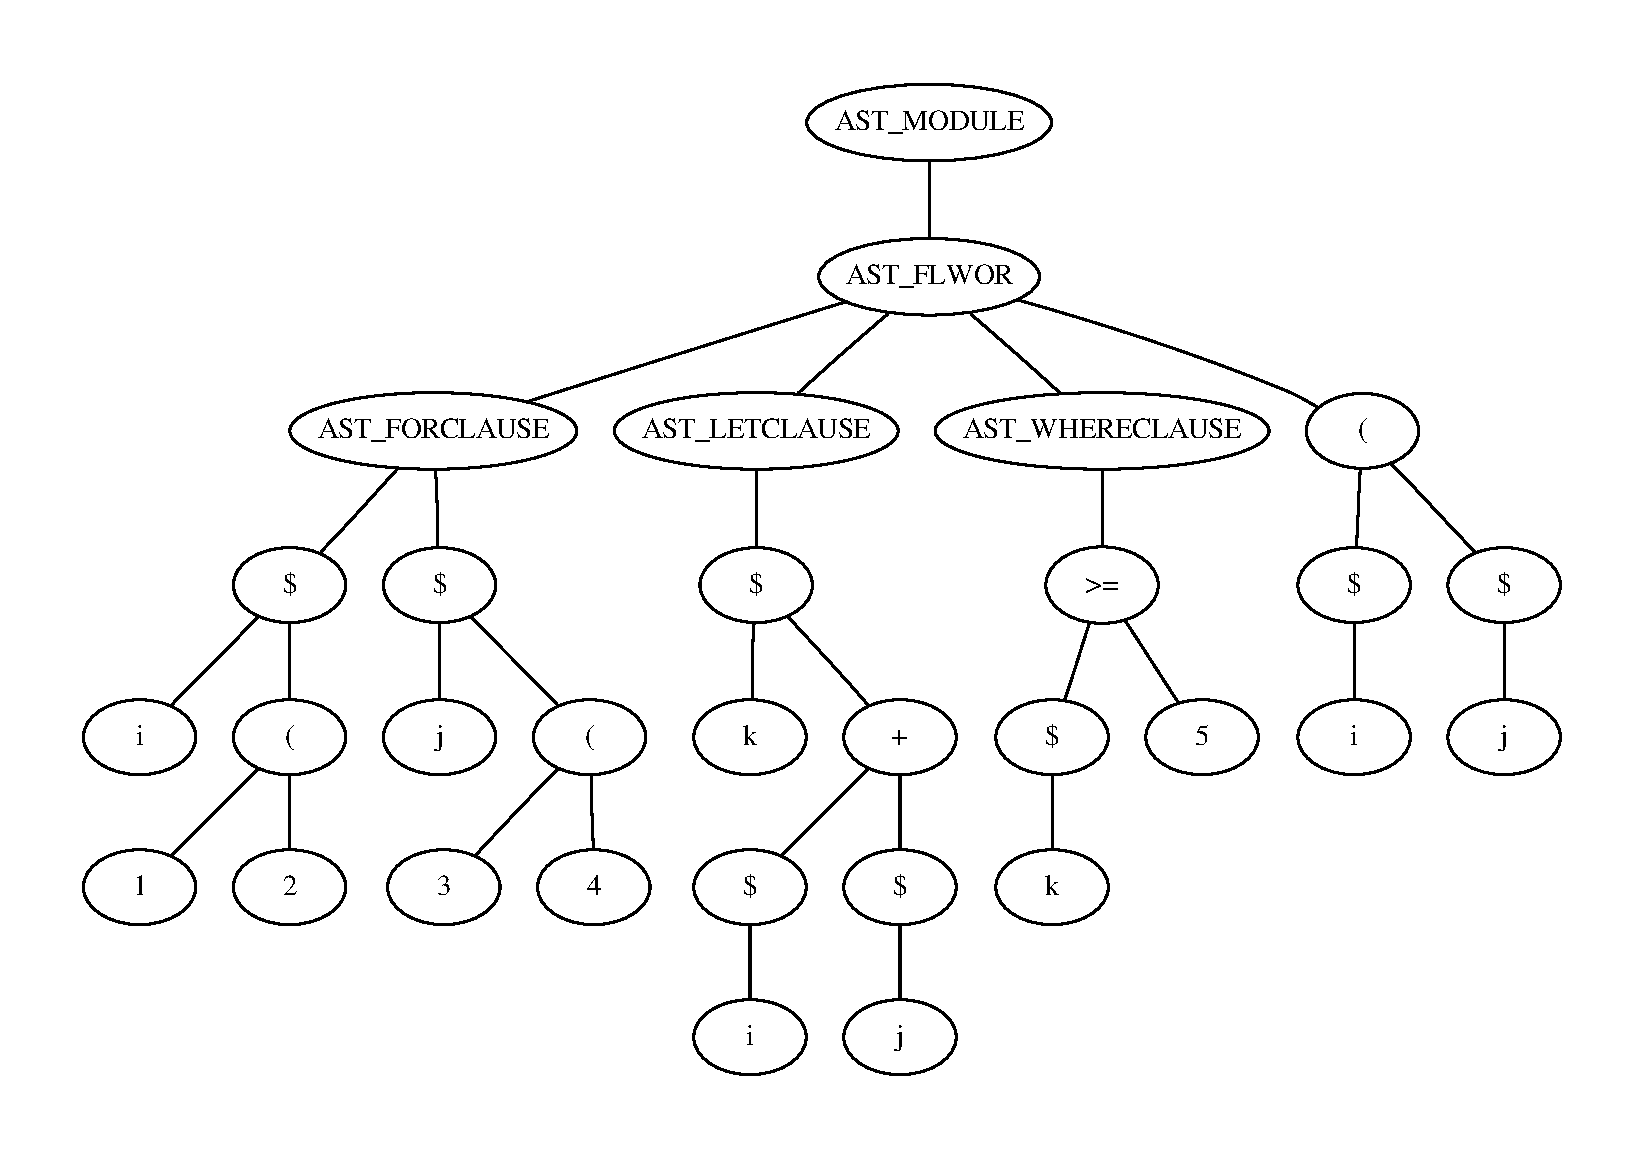
\includegraphics[scale=0.50]{img/graphs/flwor_rewrite1}
\caption{FLWOR AST tree before normalization}
\label{tree:ast:flwor_rewrite1}
\end{figure}

\begin{figure}[h!]
\centering
 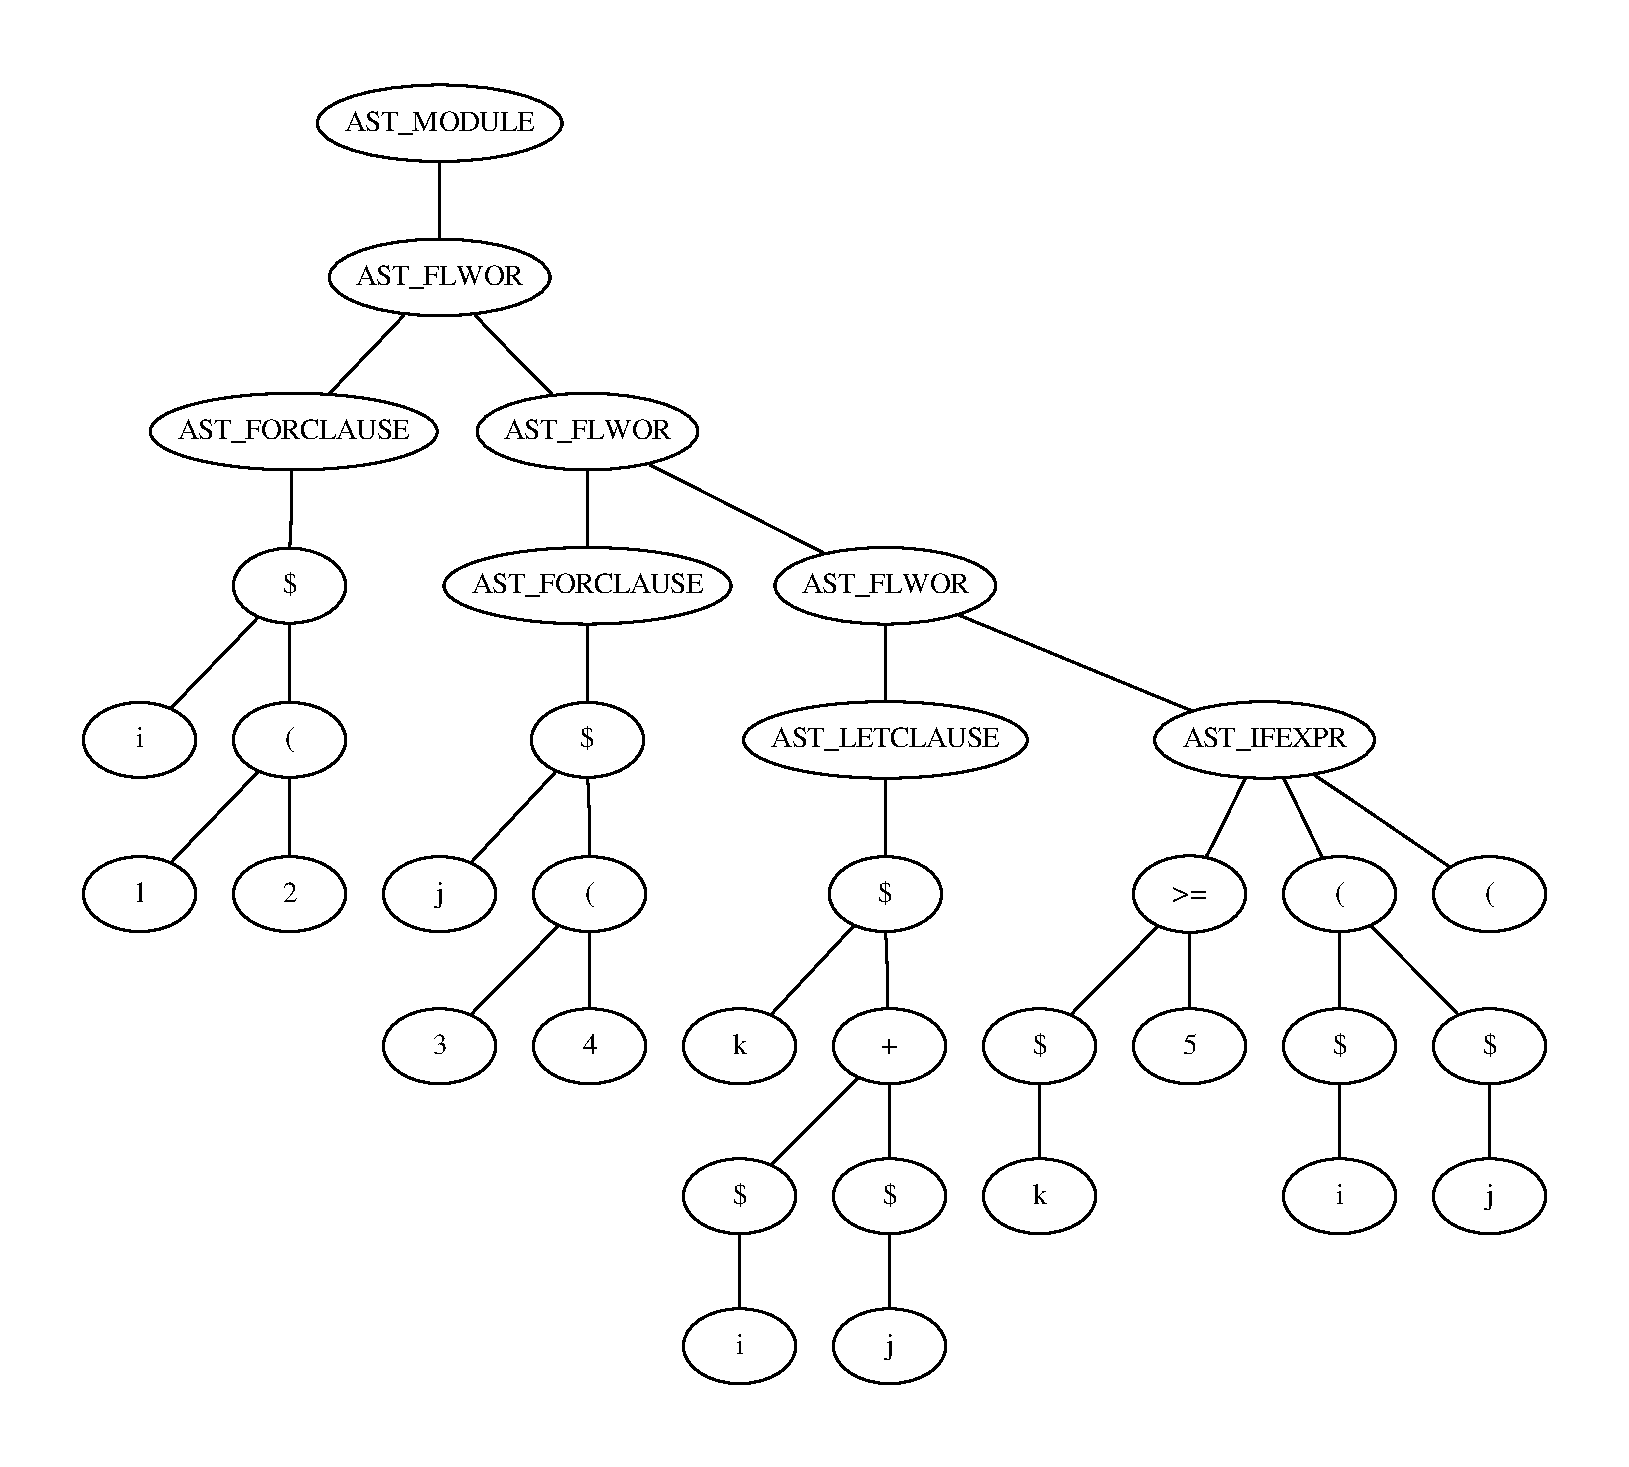
\includegraphics[scale=0.50]{img/graphs/flwor_rewrite2}
\caption{Normalized FLWOR AST tree}
\label{tree:ast:flwor_rewrite2}
\end{figure}

\subsubsection{Rewriting composite relative path expressions}
A composite relative path expression (for example, \verb!a/b!), can be
rewritten into a for loop using the mapping rule in
\ref{figure:xquery:relpath_mapping_rule}.

\begin{figure}[!h]
\centering
$[RelativePathExpr / StepExpr]_{Expr}$ \newline
$==$ \newline
fs:apply-ordering-mode ( \newline
fs:distinct-doc-order-or-atomic-sequence ( \newline
    let \$fs:sequence as node()* := $[RelativePathExpr]_{Expr}$ return \newline
    let \$fs:last := fn:count(\$fs:sequence) return \newline
    for \$fs:dot at \$fs:position in \$fs:sequence return \newline
       $[StepExpr]_{Expr}$
))
  \caption{Composite relative path expression mapping rule}
  \label{figure:xquery:relpath_mapping_rule}
\end{figure}

Given the trivial example \verb!a/b!, this translates into the following block
of normalized code:

\begin{verbatim}
fs:apply-ordering-mode (
fs:distinct-doc-order-or-atomic-sequence (
  let $fs:sequence as node()* := a return
  let $fs:last := fn:count($fs:sequence) return
  for $fs:dot at $fs:position in $fs:sequence return
    b))
\end{verbatim}

Which may seem like a rather verbose representation of such a simple path
expression. In particular, for complex path expressions this may
escalate into rather large rewritten expressions. However, this is a trade-off
to be made for normalization of such path expressions.

\subsection{AllMatches}
\label{sect:theory:xquery:allmatches}
\begin{itemize}
  \item http://www.w3.org/TR/xpath-full-text-10/\#AllMatchesSec
  \item Hva er AllMatches?
  \item Kobling til fulltekst
  \item Noen eksempler
  \item Den store forskjellen med AllMatches er at den minste enheten i et 
        dokument er et ord og ikke en tekstnode
\end{itemize}
\textbf{\underline{\LARGE TODO:}} Ikke sikkert at dette er noe poeng aa skrive
om hvis vi bare ignorerer fulltekst uansett. Kunne foreslaatt en tilnarming ala galatex kanskje, som bare
oversetter greiene til funksjonskall.
